\section{Authentication}

\subsection{JWT: JSON Web Tokens}

\subsubsection{Overview}

\begin{frame}[allowframebreaks]
	\frametitle{Overview}
	
	\begin{block}{JWT\emph{s} = \textbf{J}SON \textbf{W}eb \textbf{T}oken\emph{s}}
		\begin{itemize}
			\item Simple and stateless mean to provide authentication
			\begin{itemize}
				\item the server doesn't need to store session data
			\end{itemize}
			\item Use case:
			\setbeamertemplate{enumerate items}[default]
			\begin{enumerate}
				\item Some client POSTs username \& password to some predefined route, e.g. \texttt{/users/\{username\}/login}
				\item On valid requests, the server responds with one \emph{token}
				\begin{itemize}
					\item[N.B.] the token is \emph{signed} using some secret that never leaves the server, so the token \textbf{cannot be compromised or forged}
				\end{itemize}
				\item The client stores the token, e.g. within its \emph{local storage}
				\item Any subsequent request from the client should contain the token, e.g. within the \texttt{Authorization} header, the query or the body
				\item The server should verify the signature of every request containing one token: once validated, any \emph{claim} contained within the token can be entrusted
			\end{enumerate}
		\end{itemize}
		
	\end{block}
	
	\begin{block}{JWT - Sequence Diagram}
		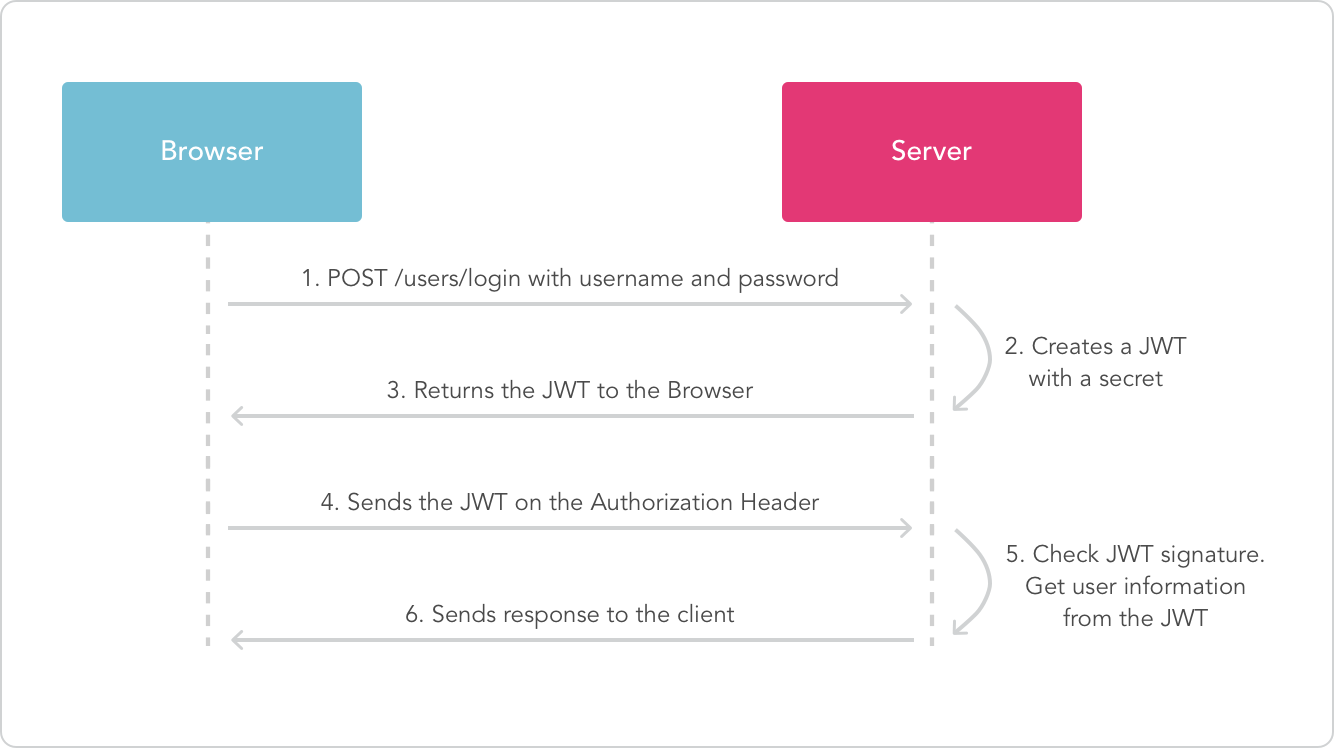
\includegraphics[width=\textwidth]{img/jwt-diagram.png}
	\end{block}
	
\end{frame}

\subsubsection{Structure}

\begin{frame}[allowframebreaks]
	\frametitle{JWT Structure}
	
	\begin{block}{JWT - Anathomy Diagram}
		\centering
		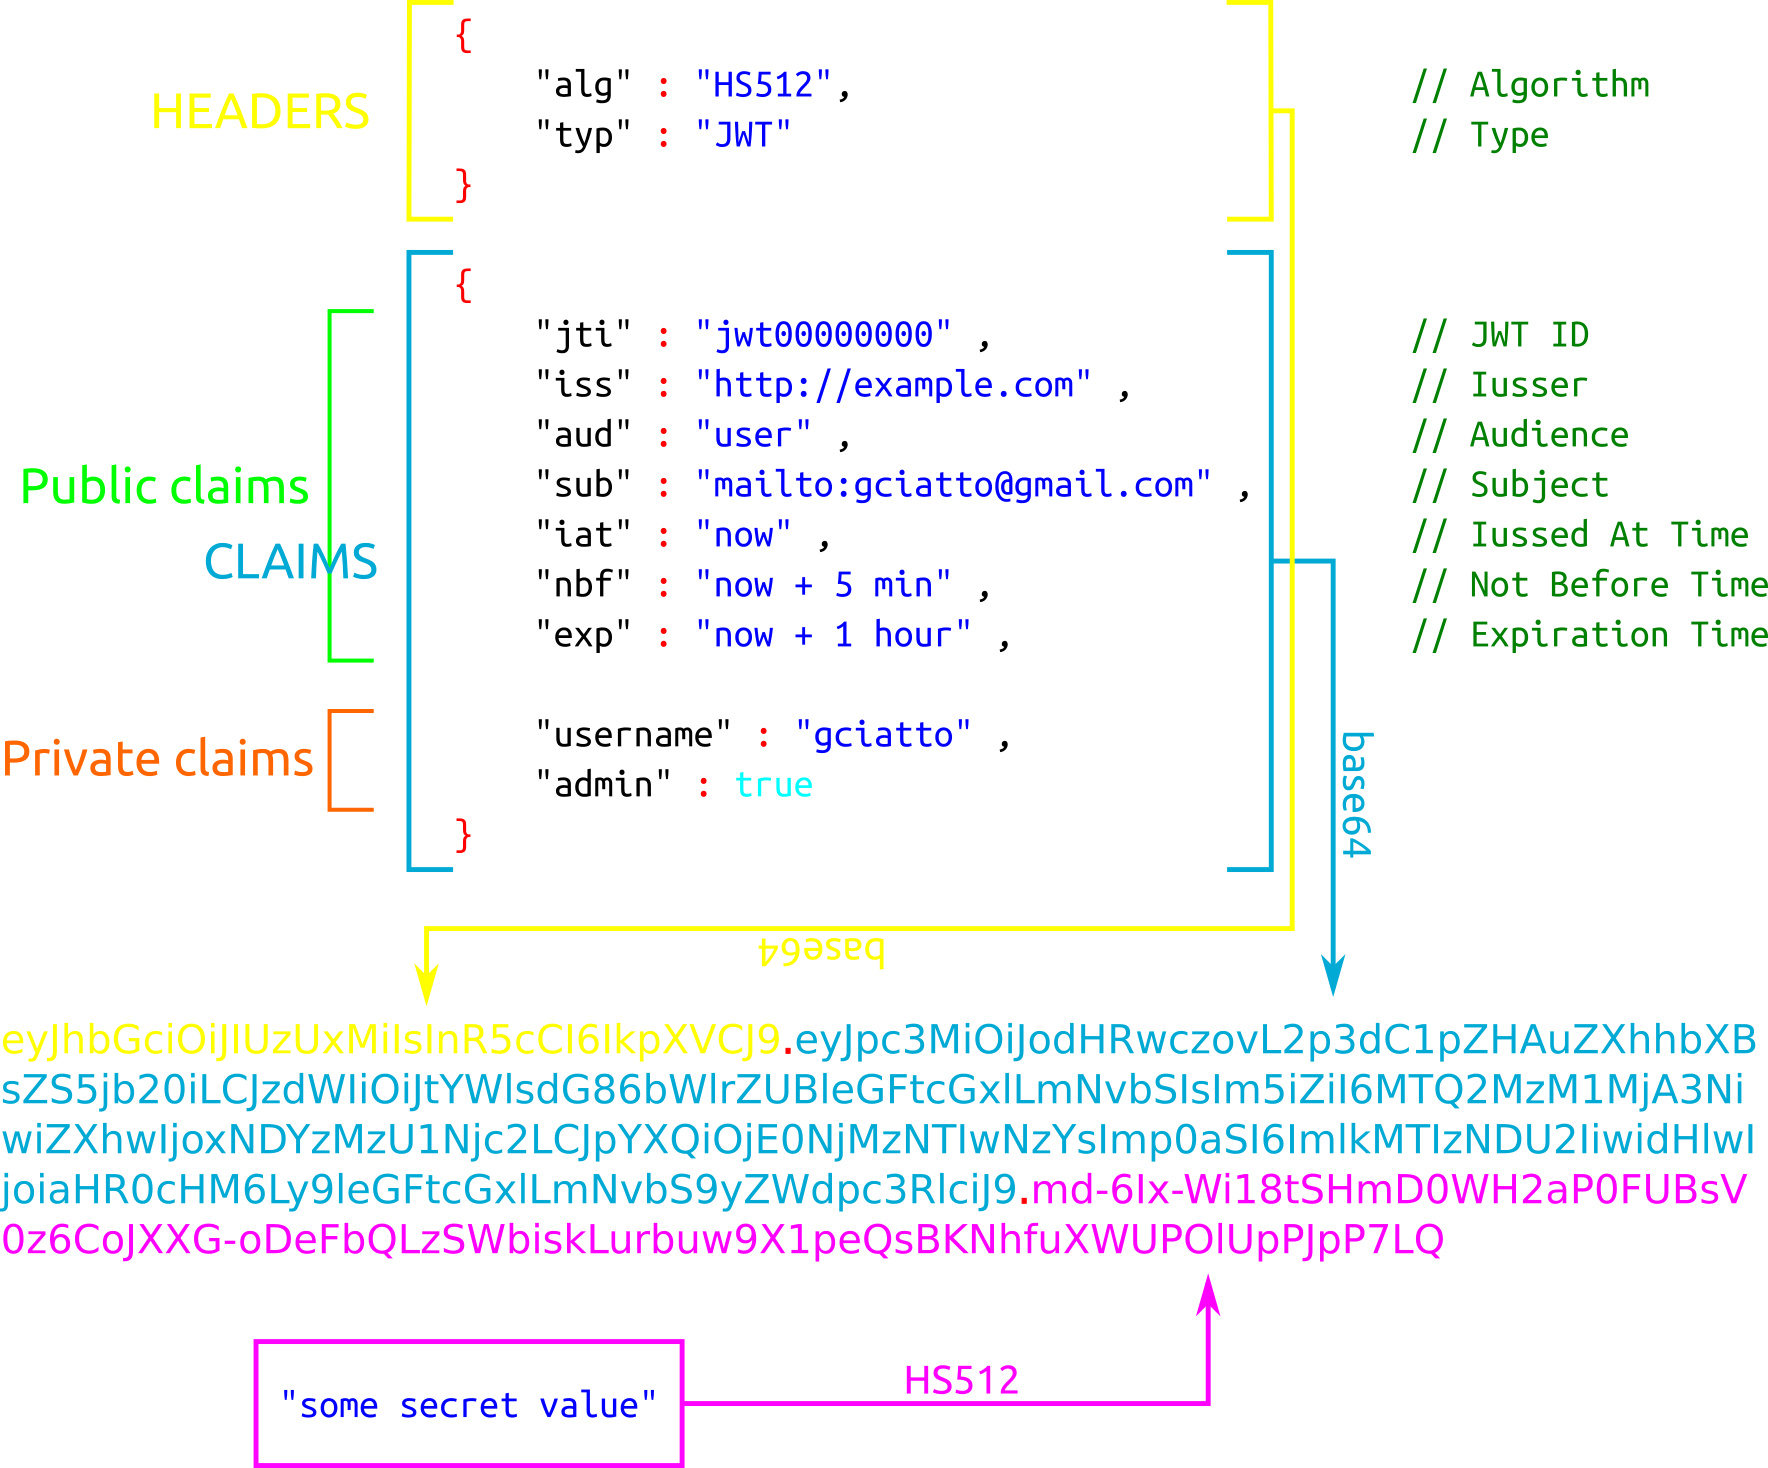
\includegraphics[height=0.7\textheight]{img/jwt.png}
	\end{block}
	
	\framebreak
	
	\begin{block}{JWT - Sections}
		\begin{itemize}
			\item Defined in \texttt{RFC 7519}
			\item String containing 3 dot-separated section
				\setbeamertemplate{enumerate items}[default]
				\begin{enumerate}
					\item The first section is a JSON object, called \emph{Headers}, \texttt{base64} encoded
					\item The second section is a JSON obect, called \emph{Claims}, \texttt{base64} encoded
					\item The third section is the \emph{Signature}, obtained using \texttt{HMAC} and some \emph{secret} string
				\end{enumerate}
		\end{itemize}
	\end{block}
	
	\begin{block}{JWT - Headers}
		\begin{description}
			\item[\texttt{typ}] (Type) : usually \texttt{"JWT"} 
			\item[\texttt{alg}] (Algorithm) : the hash algorithm used (\texttt{HS512} = \texttt{H}MAC \texttt{S}HA 512)
		\end{description}
	\end{block}
	
	\begin{block}{JWT - Public claims}
		\begin{description}
			\item[\texttt{jti}] (JWT Identifier) : identifies the entity that issued the JWT
			\item[\texttt{iss}] (Issuer) : URI of the entity issuing the token
			\item[\texttt{aud}] (Audience) : identifies the recipients that the JWT is intended for
			\item[\texttt{sub}] (Subject) : identifies the entity that is the subject of the JWT
			\item[\texttt{iat}] (Issued At) : identifies the time at which the JWT was issued
			\item[\texttt{nbf}] (Not Before) : identifies the time before which the JWT \emph{musth not} be accepted for processing
			\item[\texttt{exp}] (Expiration) : identifies the expiration time on or after which the JWT \emph{musth not} be accepted for processing
		\end{description}
	\end{block}
	
	\begin{block}{JWT - Private claims}
		\begin{itemize}
			\item They are user-defined claims
			\item REMEMBER: they are public (since the token is not encrypted) but trusted (since they are signed)
			\item E.g., within the image both username and privilege level are claimed
		\end{itemize}
	\end{block}
	
\end{frame}

